\chapter{The Genius}
\label{ch:19}



\begin{center}
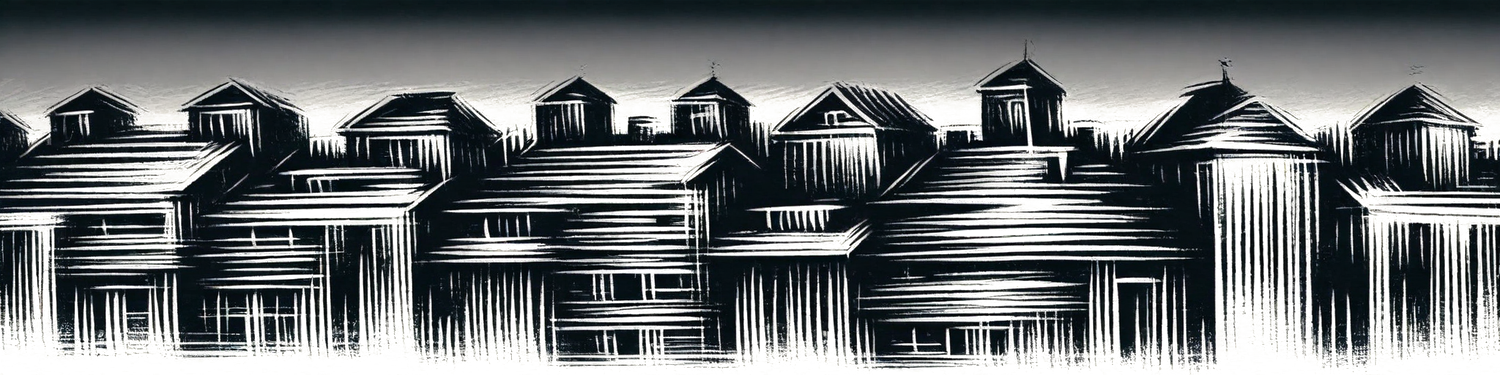
\includegraphics[width=\textwidth]{images/chapterImages/genesis_sketch_00106_.png}
\end{center}

Dr. Katherine Okonkwo's office at MIT was exactly what Sarah expected: walls covered in equations, papers stacked precariously on every surface, whiteboards filled with proofs that looked more like art than mathematics. Katherine herself was younger than Sarah had pictured—early thirties, Nigerian-American, with natural hair pulled back in a hasty bun and the kind of intense focus that made Sarah recognize a kindred spirit immediately.

"Dr. Chen," Katherine said, not getting up from her desk. "James Wei said you wanted to talk about my Fields Medal work. I have fifteen minutes."

"I need to show you something first. Then you can decide how much time you have."

Sarah pulled up her laptop. Showed Katherine the genetic timeline. The activation sequences. The correlation between cognitive capabilities and historical breakthroughs.

Katherine's expression didn't change as she studied the data. She scrolled through it methodically, checking each correlation, each timeline, each piece of evidence. Sarah had learned not to interpret silence as skepticism—brilliant people took time to process.

After ten minutes, Katherine sat back. "Show me the mathematical reasoning activation sequence."

Sarah pulled it up. The genetic markers for advanced abstract reasoning. For pattern recognition at the deepest levels. For the capacity to see relationships between concepts that seemed unrelated.

"When does this activate?"

"The first wave hit approximately 350 years ago. Newton. Leibniz. The beginning of modern calculus. Second wave about 200 years ago—multiple independent developments in non-Euclidean geometry, complex analysis, abstract algebra. Third wave about 50 years ago—"

"Category theory," Katherine interrupted. "Chaos theory. Fractal mathematics. All emerging simultaneously from different researchers."

"Yes."

"And you're saying this isn't convergent thinking. This is genetic activation. We're all expressing the same capability because the code turned it on."

"That's what the data suggests."

Katherine stood up. Went to one of her whiteboards. Stared at the equations there. Sarah recognized some of it—advanced topology, category theory, structures she'd seen in graduate school but never fully understood.

"Four years ago," Katherine said quietly, "I had a breakthrough. I was working on a problem in algebraic topology that had been unsolved for decades. Woke up one morning and just... saw it. The entire proof. Complete. I spent three weeks writing it down, but the understanding was instant."

She touched one of the equations. "It felt like remembering something I'd forgotten. Not discovering something new. Remembering."

"What did the proof show?" Sarah asked.

"A new relationship between seemingly unrelated mathematical structures. A pattern that connected topology, algebra, and number theory in ways no one had suspected. It was beautiful. Elegant. And completely unexpected."

"Did anyone else discover it simultaneously?"

Katherine turned to look at her. "Three other mathematicians published similar results within six months. We thought it was remarkable coincidence. The mathematics community loves those stories—simultaneous independent discovery. Proof that certain ideas are 'in the air,' ready to be found."

"It wasn't in the air," Sarah said. "It was in your genes. All four of you activated the same capability at the same time. Expressed the same cognitive architecture. Saw the same patterns because you were programmed to see them."

Katherine was quiet for a long time. Then she said, "Show me my genetic profile."

"I don't have your—"

"I participated in a genomics study two years ago. Published data. Here." Katherine pulled it up on her computer. Her complete genetic sequence, publicly available for research.

Sarah ran the analysis. Cross-referenced with the mathematical reasoning markers. The correlation was perfect. Katherine had every single high-expression variant. She was the genetic ideal for advanced mathematics capability.

"Ninety-ninth percentile," Sarah said. "You're in the top one percent for expression of these sequences."

"So I'm not a genius," Katherine said flatly. "I'm just early activation."

"You're both. The activation gives you capacity. What you do with it—"

"Is what? My choice? My personality?" Katherine laughed without humor. "Dr. Chen, I was five years old when I first saw mathematical patterns in everything. Flowers. Clouds. The way people arranged themselves in groups. I've been doing mathematics since before I could articulate what mathematics was. You're telling me that wasn't me? That was genetic programming?"

"The capacity was programmed. Your use of it—"

"Is determined by my neurology, which is also genetic. My obsessive focus? Genetic. My ability to visualize abstract structures? Genetic. My compulsion to work eighteen-hour days? Genetic. Where exactly is the 'me' in all of this? What part is actually Katherine and not just activated code?"

Sarah didn't have an answer. She'd been asking herself the same question about her own obsession. Her own compulsion. Her own inability to choose Maya over the work.

Katherine went back to the whiteboard. Studied her equations again. "I was so proud," she said quietly. "The Fields Medal. Youngest recipient in thirty years. Proof of my brilliance. Confirmation that all the sacrifice was worth it."

"What did you sacrifice?"

"Everything. Relationships. Health. Any semblance of normal life. I tell myself it's worth it because I'm doing something meaningful. Something only I can do. But if thousands of other people have the same genetic activation..." She trailed off.

"You're not special," Sarah finished. "You're just first."

"Yes."

"Does that make the mathematics less beautiful?"

Katherine considered this. Touched one of her equations. "No. The patterns exist independent of who discovers them. The relationships are true regardless of whether I see them or someone else does. The mathematics doesn't care about human pride."

"But you care."

"Of course I care. I'm human. Or I thought I was. Now I'm learning I'm a program that thinks it's human."

"We're all programs," Sarah said. "The question is whether the program includes genuine experience or just the illusion of it."

"You don't know, do you? You can't tell from genetics whether consciousness is real or simulated."

"No."

Katherine sat down at her desk. Pulled up more of the genetic data. Studied it with the same intensity she probably applied to her mathematical proofs. "These activation sequences—they're incredibly precise. The timing. The triggers. The cascading effects. Whoever designed this was working at a level of complexity that's..." She trailed off, scrolling through the code. "This is beautiful. This is the most elegant programming I've ever seen."

"The dinosaurs designed it."

"The dinosaurs were mathematicians," Katherine corrected. "Had to be. You can't create something this complex without deep mathematical understanding. Probably deeper than anything we've achieved." She looked up at Sarah. "We're not even close to their level. We think we're sophisticated because we can build computers and satellites. But they programmed an entire species' evolution across 65 million years using nothing but genetics. That's orders of magnitude more complex than anything we've accomplished."

"Does that make you feel better or worse?"

"I don't know yet. Ask me after I process the existential crisis."

Sarah's phone buzzed. She ignored it. Probably her ex again. Probably more about Maya. She couldn't think about that now. Couldn't handle that guilt on top of everything else.

"I need your help," Sarah said. "I'm building a team. Researchers who can verify this discovery. Who can help analyze the implications. You're one of the best mathematical minds in the world—activated or not. I need your ability to see patterns."

"To see patterns I was programmed to see."

"Does it matter where the ability comes from if it's useful?"

Katherine considered this. "What are you planning to do with this information?"

"I don't know yet. First I need to understand it fully. Then... I guess we need to decide whether humanity deserves to know they're executing code."

"They'll reject it," Katherine said immediately. "The religious implications alone. Every faith tradition is built on the assumption that humans have souls, free will, special status in creation. You're telling them they're tools built by reptiles. That'll go over great."

"So we hide it?"

"I didn't say that. I'm saying be prepared for the consequences. This knowledge will break people. Will destroy existing philosophical frameworks. Will force a complete re-evaluation of what it means to be human."

"That's why I need people like you. People who can think clearly about implications. Who can help humanity process this without mass panic."

Katherine was quiet for a long time. Sarah could see her thinking, calculating, running through scenarios with the same mathematical precision she probably applied to her proofs.

Finally: "I'm in. But not because I want to be. Because I can feel it. The compulsion. The need to understand. The inability to let this go now that I know it exists." She looked at Sarah. "Is that me choosing? Or is that activation?"

"I don't know."

"Neither do I. But I'm doing it anyway."

"Story of my life lately," Sarah muttered.

Katherine pulled up the genetic data on her screen. Started analyzing it with professional focus, the existential crisis already compartmentalized so she could work. Sarah recognized the behavior. She'd done the same thing. Had gone from devastating revelation to clinical analysis in hours.

"Question," Katherine said without looking up. "If we're programmed, and we're building planetary defense systems on schedule, what happens after? Is there a next activation? Or does the program end once we've served our purpose?"

Sarah pulled up the analysis she'd been avoiding. The sections of the code that came after the engineering capability. The sequences that were still dormant. Still waiting.

"There's more," she said. "At least three more major activation sequences. I haven't fully analyzed them yet. But they're there. Waiting for the right triggers."

"So we're not the end goal. We're a step. One threshold in a longer sequence."

"Yes."

"What are we building toward?"

"I don't know. But whoever programmed this—whatever the dinosaurs were—they were thinking longer than just solving the asteroid problem. They were planning multiple steps ahead. Setting up a cascade that goes beyond planetary defense."

Katherine looked up from her screen. "That's terrifying."

"Or inspiring. Depending on your perspective."

"Right now, I'm going with terrifying."

Sarah's phone buzzed again. She looked at it this time. Twenty-three missed calls. Seventeen messages. All from her ex and Maya's school.

"You need to get that?" Katherine asked.

"No. Yes. I don't know." Sarah put the phone away. "My daughter needs me and I'm here analyzing genetic code that proves we're all programs. What does that say about me?"

"That you're activated for research capability. That the compulsion is strong. That you're doing what you were designed to do."

"Is that supposed to make me feel better?"

"Is it making you feel better?"

"No."

"Then I'm just being accurate, not comforting."

Sarah almost laughed. "You're terrible at empathy."

"Genetic deficit. My neurology is optimized for mathematics, not emotional intelligence. See? More programming. Less free will. We're consistent, at least."

"I was trying to be there for Maya," Sarah said. "I really was. But every time I try to focus on her, the data comes back. The questions. The need to understand. It's like my brain won't let me think about anything else."

"That's the activation. The compulsion. It's not subtle. I feel it too. Right now I should be finishing a paper that's due in two weeks. Instead I'm here analyzing your genetic data because I can't not analyze it. The mathematics demands attention. It overrides everything else."

"How do you live with that?"

"I don't. I just exist in it. Work sixteen hours a day. Sleep barely. Eat when I remember. It's not living. It's executing."

Sarah looked at her phone again. At the missed calls from people who loved her or at least needed her. At the evidence of her failure to be human while proving humans were programs.

"I should go," she said.

"Will you?"

Second person today to ask her that. Second time she didn't have a real answer.

"Eventually."

"But not now."

"Not now."

Katherine nodded. Understanding. Not judging. Both of them caught in the same compulsion. Both unable to choose away from it even as they recognized it for what it was.

"I'll work on verifying the mathematical structure of the genetic code," Katherine said. "If this is real programming, it should show design patterns. Optimization. Elegant solutions to complex problems. I can identify those."

"Thank you."

"Don't thank me. I'm not doing this by choice. I'm doing it because my genetics are compelling me to. We're both just executing our code."

"Does it feel like execution?"

Katherine thought about this. "No. It feels like the most meaningful work I've ever done. It feels like discovering truth. It feels like fulfillment." She paused. "Which is probably exactly how good programming should feel. The tool should want to do its function. Should feel satisfaction in performing its designed purpose."

"That's bleak."

"That's efficient."

Sarah gathered her materials. Prepared to leave. Prepared to not leave. Prepared to drive toward Maya and end up at the lab instead.

"One more thing," Katherine said. "If we're programs executing code, and we're approaching the activation for planetary defense, that means—"

"The asteroid is coming," Sarah finished. "Yes."

"How long?"

"I don't know. But if the code is timed correctly—if whoever programmed this calculated accurately—then we're building the defense system right before we need it. Which means soon. Geologically speaking."

"How soon?"

"Within a few decades. Maybe sooner."

Katherine looked back at her equations. At the patterns she'd discovered that weren't really discoveries at all. Just activations. Just scheduled expressions of programmed capability.

"We should probably hurry then," she said.

"Probably."

Sarah left. Walked to her car. Sat in the driver's seat for ten minutes trying to decide where to go.

Maya or the lab.

Her daughter or the truth.

The person who needed her or the species that needed to understand what they were.

She started the engine.

Drove toward the lab.

Hated herself.

Did it anyway.

The program was executing.

And she was part of the execution.

Whether that was choice or compulsion, she no longer knew.

Whether the distinction mattered, she was beginning to doubt.

The equation was unfolding.

And Sarah Chen was unfolding with it.

One missed call at a time.

